\documentclass[11pt]{article}\usepackage[]{graphicx}\usepackage[]{color}
% maxwidth is the original width if it is less than linewidth
% otherwise use linewidth (to make sure the graphics do not exceed the margin)
\makeatletter
\def\maxwidth{ %
  \ifdim\Gin@nat@width>\linewidth
    \linewidth
  \else
    \Gin@nat@width
  \fi
}
\makeatother

\definecolor{fgcolor}{rgb}{0.345, 0.345, 0.345}
\newcommand{\hlnum}[1]{\textcolor[rgb]{0.686,0.059,0.569}{#1}}%
\newcommand{\hlstr}[1]{\textcolor[rgb]{0.192,0.494,0.8}{#1}}%
\newcommand{\hlcom}[1]{\textcolor[rgb]{0.678,0.584,0.686}{\textit{#1}}}%
\newcommand{\hlopt}[1]{\textcolor[rgb]{0,0,0}{#1}}%
\newcommand{\hlstd}[1]{\textcolor[rgb]{0.345,0.345,0.345}{#1}}%
\newcommand{\hlkwa}[1]{\textcolor[rgb]{0.161,0.373,0.58}{\textbf{#1}}}%
\newcommand{\hlkwb}[1]{\textcolor[rgb]{0.69,0.353,0.396}{#1}}%
\newcommand{\hlkwc}[1]{\textcolor[rgb]{0.333,0.667,0.333}{#1}}%
\newcommand{\hlkwd}[1]{\textcolor[rgb]{0.737,0.353,0.396}{\textbf{#1}}}%
\let\hlipl\hlkwb

\usepackage{framed}
\makeatletter
\newenvironment{kframe}{%
 \def\at@end@of@kframe{}%
 \ifinner\ifhmode%
  \def\at@end@of@kframe{\end{minipage}}%
  \begin{minipage}{\columnwidth}%
 \fi\fi%
 \def\FrameCommand##1{\hskip\@totalleftmargin \hskip-\fboxsep
 \colorbox{shadecolor}{##1}\hskip-\fboxsep
     % There is no \\@totalrightmargin, so:
     \hskip-\linewidth \hskip-\@totalleftmargin \hskip\columnwidth}%
 \MakeFramed {\advance\hsize-\width
   \@totalleftmargin\z@ \linewidth\hsize
   \@setminipage}}%
 {\par\unskip\endMakeFramed%
 \at@end@of@kframe}
\makeatother

\definecolor{shadecolor}{rgb}{.97, .97, .97}
\definecolor{messagecolor}{rgb}{0, 0, 0}
\definecolor{warningcolor}{rgb}{1, 0, 1}
\definecolor{errorcolor}{rgb}{1, 0, 0}
\newenvironment{knitrout}{}{} % an empty environment to be redefined in TeX

\usepackage{alltt}

\usepackage{rotating}
\usepackage{graphics}
\usepackage{latexsym}
\usepackage{color}
\usepackage{listings}
\usepackage{wrapfig}
\usepackage{float}
\usepackage[belowskip=-15pt,aboveskip=0pt]{caption}

\setlength\topmargin{-.56in}
\setlength\evensidemargin{0in}
\setlength\oddsidemargin{0in}
\setlength\textwidth{6.49in}
\setlength\textheight{8.6in}
\setlength{\intextsep}{10pt plus 1pt minus 4pt}

\definecolor{codegreen}{rgb}{0,0.6,0}
\definecolor{codegray}{rgb}{0.5,0.5,0.5}
\definecolor{codepurple}{rgb}{0.58,0,0.82}
\definecolor{backcolour}{rgb}{0.95,0.95,0.92}
\lstdefinestyle{mystyle}{
	backgroundcolor=\color{backcolour},   
	commentstyle=\color{codegreen},
	keywordstyle=\color{magenta},
	numberstyle=\tiny\color{codegray},
	stringstyle=\color{codepurple},
	basicstyle=\footnotesize,
	breakatwhitespace=false,         
	breaklines=true,                 
	captionpos=b,                    
	keepspaces=true,                 
	numbers=left,                    
	numbersep=5pt,                  
	showspaces=false,                
	showstringspaces=false,
	showtabs=false,                  
	tabsize=2
}
\lstset{style=mystyle}

\pagestyle{headings}

\title{Statistical Analysis and Predictive Models for Expenditures in New York Municipalities\vspace{-5ex}} 
\date{October 08, 2020\vspace{-5ex}}
\IfFileExists{upquote.sty}{\usepackage{upquote}}{}
\begin{document} 
\maketitle








\noindent\textbf{\underline{Executive Summary}} 
\hfill \break

\noindent\textbf{\underline{Introduction}} 

\noindent Generally, construction companies have numerous aspects in estimating the cost of each new housing project. To estimate the cost of each housing project, expenditures play an important role in increasing or decreasing the cost. For example, higher expenditure would result in an increase in cost of construction. Therefore, the property owners would have to seek for higher funding to fulfill the project. On the other hand, while expenditure decreases, property’s owner could spend the reimburse the expenses elsewhere. In addition, knowing the expenditures would also help construction manager to order supplies in a proper manger. If expenditure decreases, then the supplies would also be less in quantity or cheaper in quality. Numerous questions were proposed in favor of these issues such as 1) What variables causes the fluctuation of expenditure? 2) What is the best predictive model that could predict expenditures? 3) How can we validate and implement the model? 3) How accurate is the model? 4) Is there any improvement to the future models? To answer these questions, this analysis will take a deep dive into the data exploratory analysis, model development process using linear regression, and diagnostics analysis. With the answered questions, construction workers and properties owner would have a better understanding of their expenditures when starting a new project to avoid over or underestimating their budgets.
\hfill \break

\noindent\textbf{\underline{Methods}} 

\noindent A dataset from two New York municipalities (Warwick and Monroe) were provided to access the important measures to predict expenditures. These data contain a total of 916 observations from 1992 with 2 observation contains missing expenditure value. Two observation with NA expenditures have been removed from the analysis to improve the assumption of linear regression modeling. In terms of variables, this dataset contains three identifiers including identity number, state code, and county code and six demographic and income-related variables including wealth per person, population, percent intergovernmental, density, mean income per person, and growth rate. There is a total of 57 distinct county code implying there are multiple measurement of expenditure per county in New York. The goal of this data analysis is to predict the chances in expenditures of two New York municipalities, Warwick and Monroe. A projection dataset for Warwick and Monroe was also provided to generate predictions from using the fitted model. To achieve this goal, all analysis will be done using multiple linear regression models for model development process and accompany by diagnostics process to check for the quality of the model. All analysis including coding and writing report is done in R Studio with R version 3.6.2.    
\hfill \break

\noindent\textbf{\underline{Exploratory Data Analysis}} 

\noindent During the exploratory analysis process, it is important to access all the significant relationship of each variable with the target variable. Initially, looking at Table~\ref{descrips}, the summary statistics of all independent variables and target variable shows the maximum for expenditures, wealth, population, pint, density, income, and growth rate are extremely high compare to their mean and 75 percentiles. This indicates that all the variables mention previous are heavily right skewed. Most importantly, expenditure's skewness violates the normality assumption when generating a linear regression. Therefore, a log transformation was applied to expenditure to normalize the distribution of the target variable. Log-transformation would reduce the values which would account for outliers. Figure~\ref{inital-explore}.1. depicts the normality of the outcome variable expenditure after transformation with an overplayed of the approximately normal distribution.

\begin{figure}[h!] 
\begin{center}

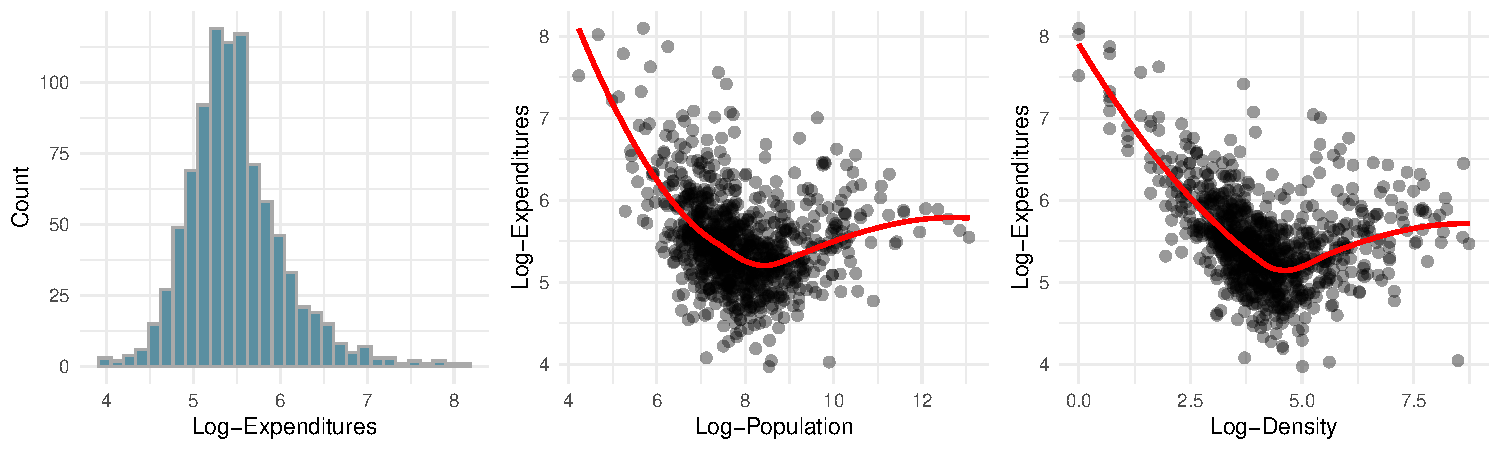
\includegraphics[width=\maxwidth]{figure/unnamed-chunk-1-1} 

\caption{Initial Exploratory Plots after Log-Transformation 1: Histogram of Log-Expenditures with Density curve in red, 2: Scatter plot of Log-Expenditures vs Log-Population with LOESS smooth line in red, and 3: Scatterplot of Log-Expenditures vs Log-Density with LOESS smooth line in red.}
\label{inital-explore}
\end{center} 
\end{figure}

\noindent Since all independent variable are right-skewed, a log-transformation also applied to each variable to ensure linear relationship with expenditures. An amount of 1.01 was added to all growth rate values to account for zeros values while taking logarithm. All variables mentioned in the rest of this article are log-transformed variables unless otherwise specified. With that being said, wealth, intergovernmental funds, income, and grow rate seems to have linear relationship with expenditures. However, population and density have different two different trend of expenditures within their plots. Figure~\ref{inital-explore}.2. shows a scatterplot of expenditures and population with a dip at approximately 8.3 to change direction of correlation. Population is self-explanatory variable which represent the number of people living in the county during the year. While population is less than 8.3, as population increases, expenditures decrease on average. When population is greater than 8.3, expenditures increase as population increases. Similar issue happens to density at 4.5, see Figure~\ref{inital-explore}.3. Density, here, represent the population of other substances like animals, environment, or other objects. To account for this problem, the data set of New York city will be subsetted into different groups according to each trend. Subsetting data will help the relationship between density and population and expenditures be linear. This analysis will only model data when population is greater than 8.3 and density is greater than 4.5 since the projection data is within these ranges.    



\noindent After selecting a subset of data, a second round of data exploratory was conducted to ensure the relationship of each measure if significant to the outcome variable expenditures. Expenditures and wealth have a positive relationship indicating the increases of wealth would cause expenditure to be higher, see Figure~\ref{sec-explore}.1. Intuitively, this makes sense since wealthier individuals would spend more resulting in higher expenses. Similarly, Figure~\ref{sec-explore}.2. shows a strong positive correlation between expenditure and income. This relationship is expected since the mean income per person is higher, their expenses would also be higher compared to lower income individuals. Other variables like population and density seem to have moderate positive relationship with expenditure, see the first two plots in Figure~\ref{sec2-explore}. Clearly, population and density are important measurements to predict expenditures. As population and density increases, the amount of expenses also increases, on average. On the other hand, predictors including intergovernmental funds and growth rate have moderate negative correlation with expenditures. This indicate that, while intergovernmental funds and growth rate increases, the amount of expenses should decrease. This makes perfect sense since if the growth rate in economic is slow, then there would be lower expenses.             

\begin{figure}[h!] 
\begin{center}

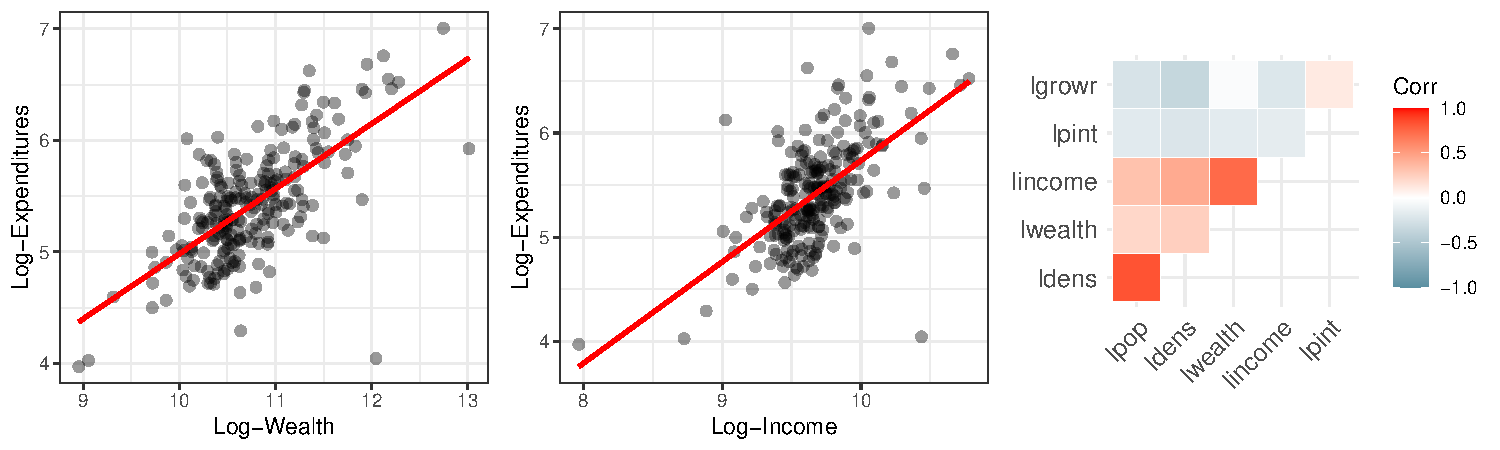
\includegraphics[width=\maxwidth]{figure/unnamed-chunk-3-1} 

\caption{Exploratory Plot after Log-Transformation and Subsetted Data 1: Scatterplot of Log-Expenditures vs Log-Wealth with Linear Regression line in red, 2: Scatterplot of Log-Expenditures vs Log-Income with linear regression line in red, and 3: Upper Correlation plot of all independent variables.}
\label{sec-explore}
\end{center} 
\end{figure}

\noindent After detecting the relationship of each independent variables with expenditures, it is important to examine the correlation of each predictors. Higher correlation between predictors mean there might be multicollinearity issues when including both variables in the model. This leads the model to have unstable and unreliable coefficients. Figure~\ref{sec-explore}.3. shows the upper diagonal of the correlation matrix plot. As one can see, density and population have a high positive correlation of 0.83. To solve the multicollinearity issues, separate models with density in one and population in other, along with other variables, were generated. The results of the models will be compared and selected as the best model. Furthermore, wealth and income also have high positive correlation of 0.74. Similar solution mentioned previously will also be applied to wealth and income. Other variables not mentioned above have little to no relationship with expenditures.          


\hfill \break

\noindent\textbf{\underline{Statistical Analysis}}
\hfill \break

\noindent\textbf{\underline{Conclusion}}
\hfill \break


\clearpage
\newpage
\noindent \Large{{\bf Appendix A: Supplemental Tables and Figures}}

\begin{center}

% Table created by stargazer v.5.2.2 by Marek Hlavac, Harvard University. E-mail: hlavac at fas.harvard.edu
% Date and time: Tue, Oct 06, 2020 - 5:14:58 PM
\begin{table}[H] \centering 
  \caption{Summary Statistics for all numerical independent features} 
  \label{descrips} 
\begin{tabular}{@{\extracolsep{5pt}}lccccccc} 
\\[-1.8ex]\hline 
\hline \\[-1.8ex] 
Statistic & \multicolumn{1}{c}{N} & \multicolumn{1}{c}{Mean} & \multicolumn{1}{c}{St. Dev.} & \multicolumn{1}{c}{Min} & \multicolumn{1}{c}{Pctl(25)} & \multicolumn{1}{c}{Pctl(75)} & \multicolumn{1}{c}{Max} \\ 
\hline \\[-1.8ex] 
expen & 914 & 293.818 & 269.678 & 53 & 172 & 316 & 3,286 \\ 
wealth & 914 & 51,837.720 & 55,994.250 & 7,744 & 25,745.2 & 54,224.8 & 594,758 \\ 
pop & 914 & 7,090.270 & 26,417.210 & 69 & 1,258.8 & 4,816.8 & 471,283 \\ 
pint & 914 & 19.231 & 10.225 & 1.700 & 12.400 & 23.975 & 68.600 \\ 
dens & 914 & 189.495 & 534.188 & 1 & 30 & 111 & 6,252 \\ 
income & 914 & 12,724.960 & 4,250.423 & 2,884 & 10,336.8 & 13,867.5 & 48,021 \\ 
growr & 914 & 8.100 & 17.434 & $-$54.100 & $-$0.300 & 13.700 & 294.500 \\ 
lexpen & 914 & 5.491 & 0.558 & 3.970 & 5.147 & 5.756 & 8.097 \\ 
lwealth & 914 & 10.599 & 0.627 & 8.955 & 10.156 & 10.901 & 13.296 \\ 
lpop & 914 & 7.876 & 1.143 & 4.234 & 7.138 & 8.480 & 13.063 \\ 
lpint & 914 & 2.826 & 0.522 & 0.531 & 2.518 & 3.177 & 4.228 \\ 
ldens & 914 & 4.141 & 1.296 & 0.000 & 3.401 & 4.710 & 8.741 \\ 
lincome & 914 & 9.409 & 0.278 & 7.967 & 9.243 & 9.537 & 10.779 \\ 
lgrowr & 914 & 1.264 & 1.925 & $-$4.009 & $-$0.270 & 2.689 & 5.689 \\ 
\hline \\[-1.8ex] 
\end{tabular} 
\end{table} 

\end{center} 

\begin{figure}[h!] 
\begin{center}

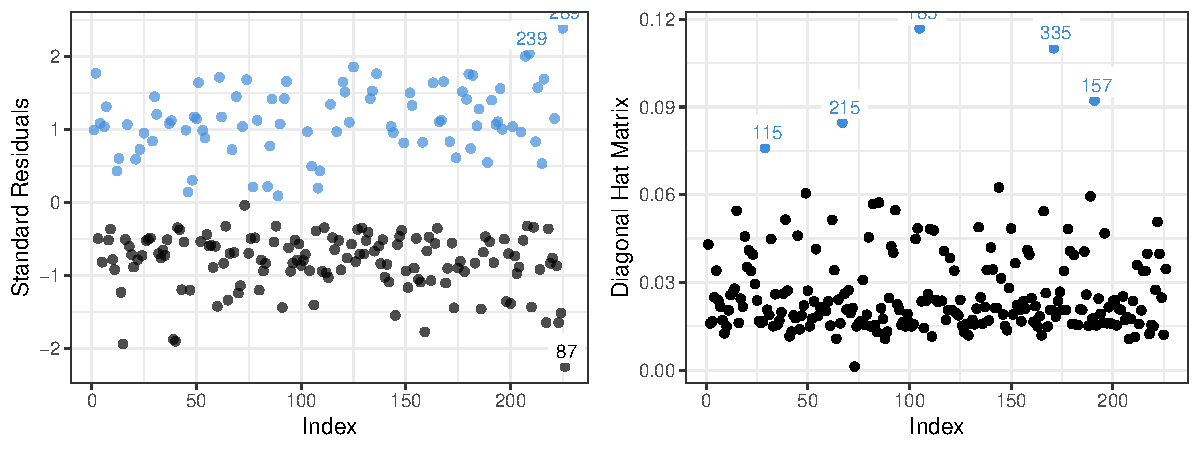
\includegraphics[width=\maxwidth]{figure/unnamed-chunk-5-1} 

\caption{Exploratory Plot after Log-Transformation and Subsetted Data 1 with linear regression line in red: 1: Log-Expenditures vs Log-Population, 2: Log-Expenditures vs Log-Intergovernmental FUnds, 3: Log-Expenditures vs Log-Density, and 4: Log-Expenditures vs Log- Growth Rate.}
\label{sec2-explore}
\end{center} 
\end{figure}


\end{document}






